\documentclass[a4paper,12pt]{article}

\usepackage[backend=biber]{biblatex}
\bibliography{report.bib}

\usepackage{circuitikz}
\usetikzlibrary{shapes}

\usepackage{graphicx}
\DeclareGraphicsExtensions{.pdf}

\usepackage{fancyhdr}
\pagestyle{fancy}
\fancyhf{}
\rhead{Dominic Moylett - dm1905@my.bristol.ac.uk}
\cfoot{Page \thepage}

\usepackage{listings}
\definecolor{comment}{HTML}{75715E}

\begin{document}
    \begin{center}
        \section*{Fault Tolerant Computing and VLSI Testing}
        \subsection*{Individual Project:\\Self-Purging Redundancy on a MIPS ALU Unit}
    \end{center}

    \section{Introduction}

    Fault tolerant circuit design has become increasingly important over the past several decades, due to the demand for faster and smaller systems. A common method for making circuits tolerate one of the modules developing a fault is through redundancy: having multiple instances of the same module and taking the vote as the majority verdict. A system with N modules has N Module Redundancy (NMR).

    Following on from NMR, development began on hybrid techniques. These techniques often involve more complex logic to ensure the system functions correctly even after more than the majority of modules develop faults. Examples include NMR-with-Spare, and Self-Purging Redundancy (SPR) \cite{1674656}. The latter will be the focus of this report.

    I investigate self-purging redundancy by implementing it on the ALU of a MIPS processor. I explain the logic for SPR and compromises made. Mathematical models are used to measure the reliability depending on the number of modules and the voter threashold. The circuit was synthesised by the Synopsys Design Compiler and metrics for area, timing and power were taken. From these results, I reach a compromise between reliability and overhead and compare with both the original circuit and NMR circuits. The Verilog source code for the final self-purging redundancy scheme is included as part of this submission, the modified file being mipsparts.v.

    Also included in this report is the script used to generate the metrics.

    \section{Realisation of Self-Purging Redundancy}
    \label{sec:realisation}

    NMR circuits decide on their output by using a voter circuit, which checks if one value is produced by the majority of modules. This is done by testing all ${n \choose k}$ combinations of modules where $n$ is the number of modules and $k = \lceil\frac{n}{2}\rceil$ is the number of modules required for a majority.

    An example is below for three modules $a, b, c$ and output $r$:

    $$r = ab + ac + bc$$

    And again for five modules $a, b, c, d, e$:

    $$r = abc + abd + abe + acd + ace + ade + bcd + bce + bde + cde$$

    For $r = 1$, a majority of modules must output 1.

    SPR on the other hand uses a more general 'threashold voter'. A threashold voter produces $r = 1$ if at least $k$ modules produce $1$, where $k \in \{2,...,n-1\}$. The version with three modules is the same as before, but for five modules we can now use the following logic for a threashold of two:

    $$r = ab + ac + ad + ae + bc + bd + be + cd + ce + de$$

    This means that we no longer need the majority of modules to agree.

    In a traditional NMR, this would not work; if more than two modules developed faults then a failure could occur. SPR avoids this by how it handles faulty voters. Instead of allowing them to vote, a 'switch' is used to set that module's vote to $0$, preventing it from changing the outcome.

    This is typically achieved using an SR flip-flop driven by the system clock, as illustrated by Losq \cite[Section 2-B]{1674656}. Realising this in Verilog however is difficult. Firstly, because the ALU circuit receives no clock input and is instead driven by the pins themselves. And secondly, because Verilog's registers are D flip-flops, meaning that we cannot simply drive a reset signal.

    For realisation the following compromises were therefore made:

    \begin{itemize}
        \item To avoid the changes required to add a clock to the ALU, the flip-flops were instead driven by the voter output.
        \item To use D flip-flops, an XOR gate was used to set the flip-flop to $0$, an extra AND gate was used to ensure that once the switch was set to $0$ it could not be set back to $1$.
    \end{itemize}

    An example of these modifications for a simple module m and a D flip-flop d can be seen below. For simplicity, driving pins and other instances of m have been removed. At initialisation, d is set to $1$.

    \begin{circuitikz}
        \node (in) at (0,0) {};
        \node[rectangle,draw,thick,minimum width=30,minimum height=40] (m) at (2,0) {m};
        \node[and port] (result) at (5,0) {};
        \node[circle,draw,thick,minimum width=40,minimum height=40] (voter) at (9,0) {voter};
        \node[xnor port, rotate=180] (err) at (6, 2) {};
        \node[and port, rotate=180] (reset) at (4,2) {};
        \node[rectangle,draw,thick,minimum width=30,minimum height=40] (d) at (2,2) {d};
        \node (out) at (11, 0) {};
        \draw[->] (in) -- (m);
        \draw[->] (m) -| (result.in 2);
        \draw[->] (voter) -- (out);
        \draw[->] (d) -- (1,2) |- (2,1) -| (result.in 1);
        \draw[->] (result.out) -- (voter);
        \draw[->] (result.out) -| (err.in 1);
        \draw[->] (voter) -- (10, 0) |- (err.in 2);
        \draw[->] (2,1) -| (reset.in 1);
        \draw[->] (err.out) |- (reset.in 2);
        \draw[->] (reset.out) -- (d);
    \end{circuitikz}

    Another interesting question raised from this work was how to move from modules with single-bit outputs, such as the one above, to modules with multiple outputs, such as our ALU unit which has a 32-bit output pin for the result and a single-bit output pin for zero. The solution used was to treat each output bit independently with its own voting circuit and switch, though another solution could be to switch off the entire module if any of its outputs fail. This was not attempted due to time constraints.

    Using the above design for the switch and the logic for the voter specified above, the new ALU was designed in Verilog and synthesised using Synopsys Design Compiler. The design was tested for three to eleven modules, with voter threasholds ranging from two to $n-1$ for $n$ modules.

    \section{Design Compiler Script}

    The following script was used in Design Vision to synthesise the ALU circuit and measure its performance. The comment represents a command using the GUI menu items, as opposed to a shell command.

    \begin{lstlisting}[language=Bash,
        commentstyle=\color{comment}]
        #design_vision->File->Read mipsparts.v
        current_design alu
        compile
        report_timing
        report_area
        report_power
    \end{lstlisting}

    \section{Results}

    \subsection{Reliability of Self-Purging Redundancy}
    \label{subsec:equation}

    For measuring the reliability of the SPR scheme, the following equation was used from Loch \cite[~Section 3-A]{1674656}.

    $$R_{N,K}(T) = \sum_{i = K}^{N} {N \choose i}\left[R(t)\right]^i\left[1 - R(t)\right]^{N - i} $$

    N.B. this formula assumes perfect voter and switch coverage. It was not used due to complexity, but there is another formula which takes into account faults in the voter \cite[~Section 3-B]{1674656}.

    \subsection{Results for Different Threasholds}
    \label{subsec:threasholds}

    Pictured below is the reliability for the ALU over time calculated using the equation in Section~\ref{subsec:equation} for a failure rate of $\lambda = 0.001$ using the standard reliability model of $R_M(t) = e^{-\lambda t}$, for a self-purging redundancy system consisting of five modules with a voter threashold ranging from two to four modules. Also shown is the area, time and power for the same circuits.

    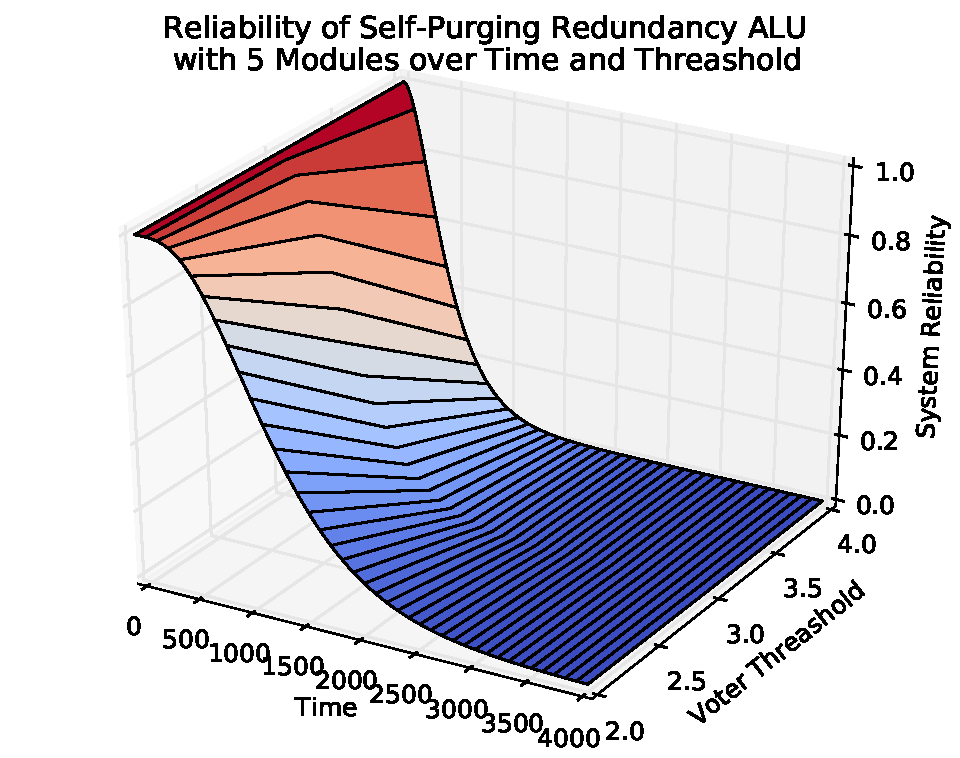
\includegraphics[width=0.5\textwidth]{reliability_5}
    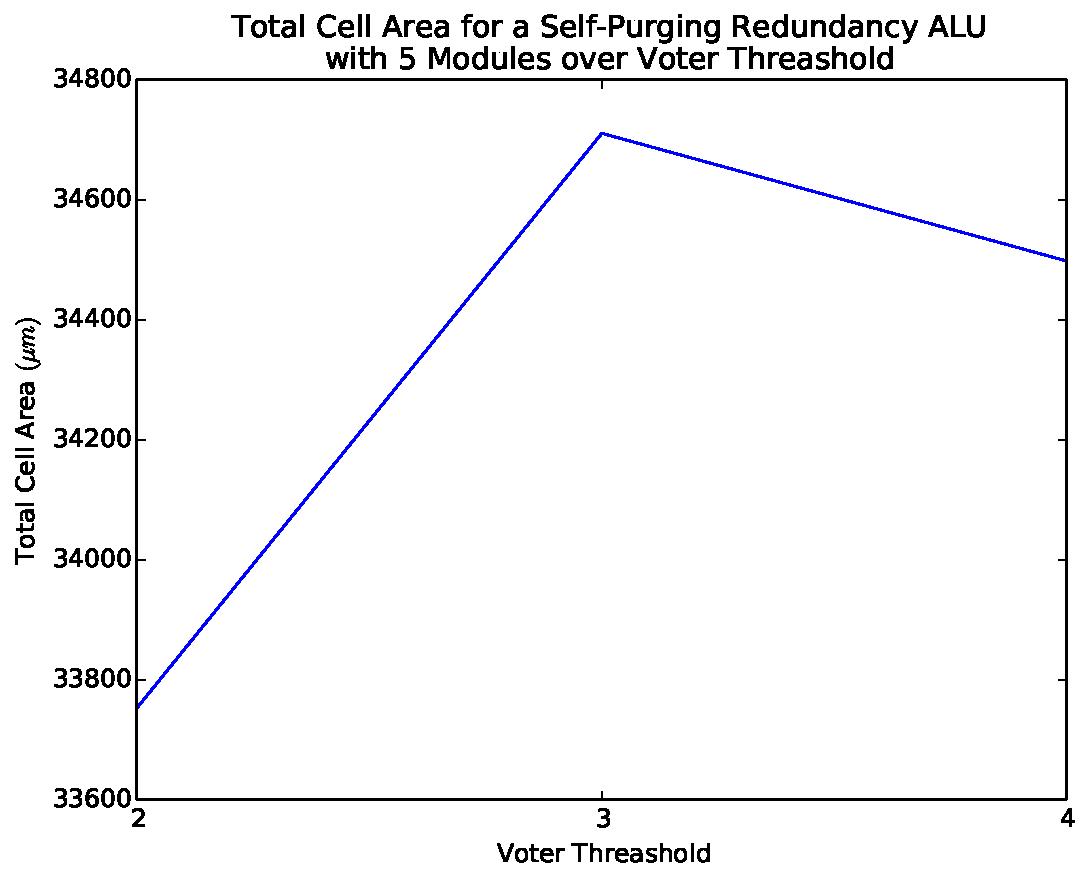
\includegraphics[width=0.5\textwidth]{area_5}

    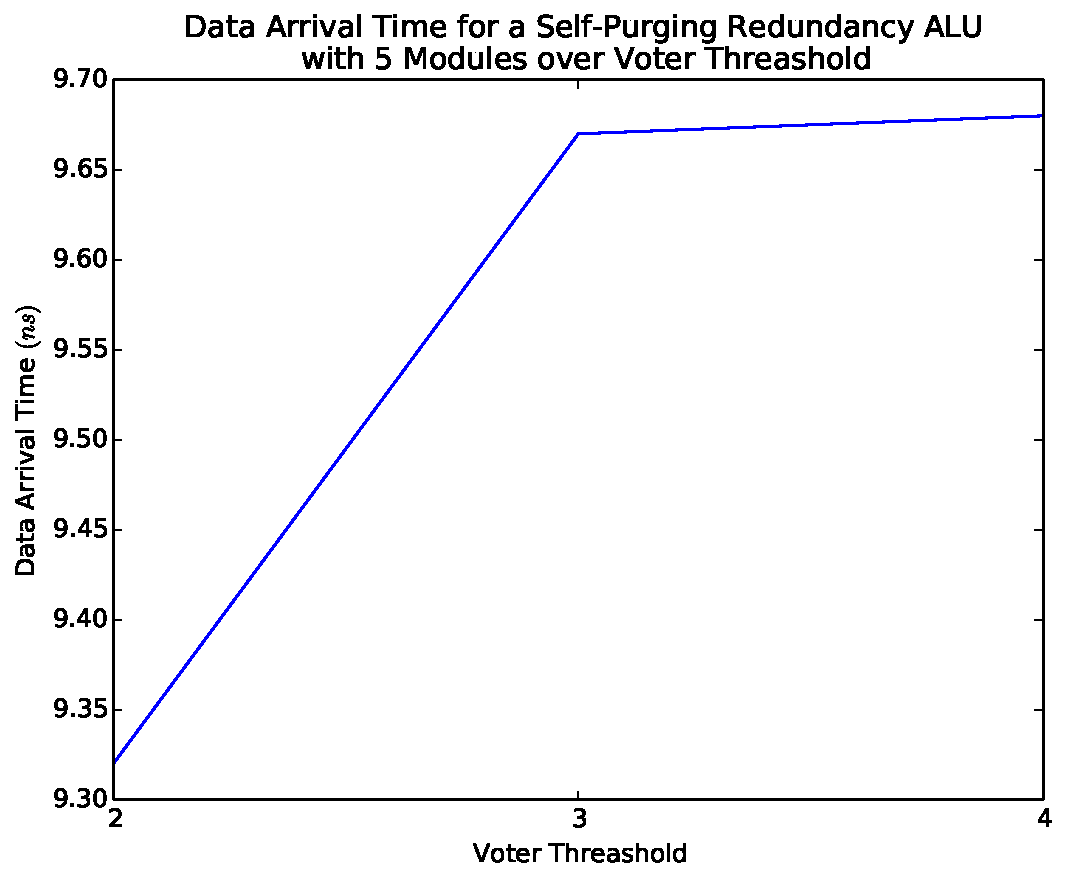
\includegraphics[width=0.5\textwidth]{time_5}
    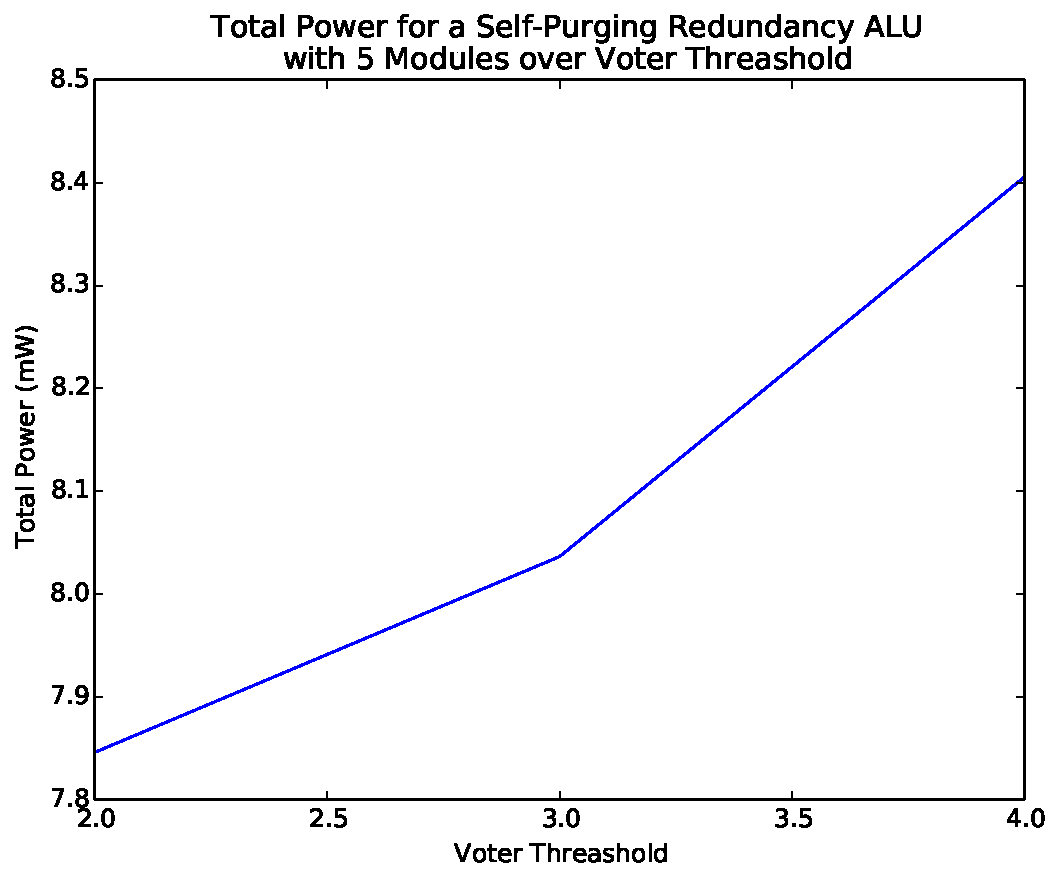
\includegraphics[width=0.5\textwidth]{power_5}

    It is clear from these results that for five modules, a voter threashold of 2 is the best choice. This is intuitive; it can be seen from the reliability formula above that the lower the threashold, the higher the reliability. Plus a voter with a threashold of 2 requires simpler logic than one with a higher threashold, so the metrics will be smaller too.

    For safety, I also measured the same metrics for a system with 11 modules, with voter threashold ranging from 2 to 10.

    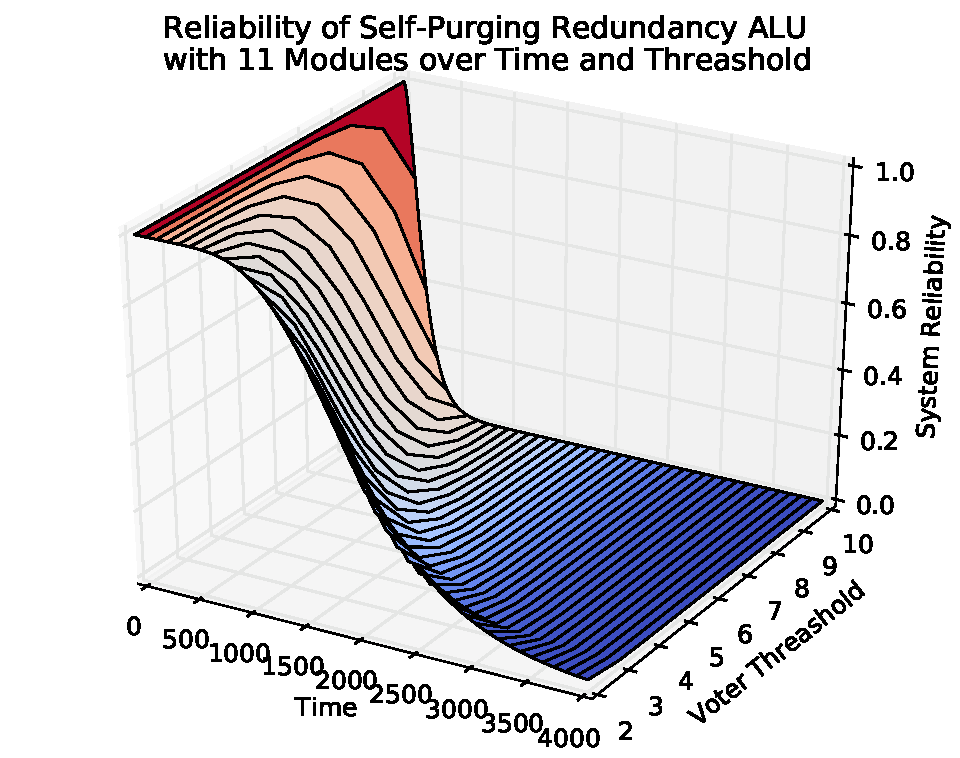
\includegraphics[width=0.5\textwidth]{reliability_11}
    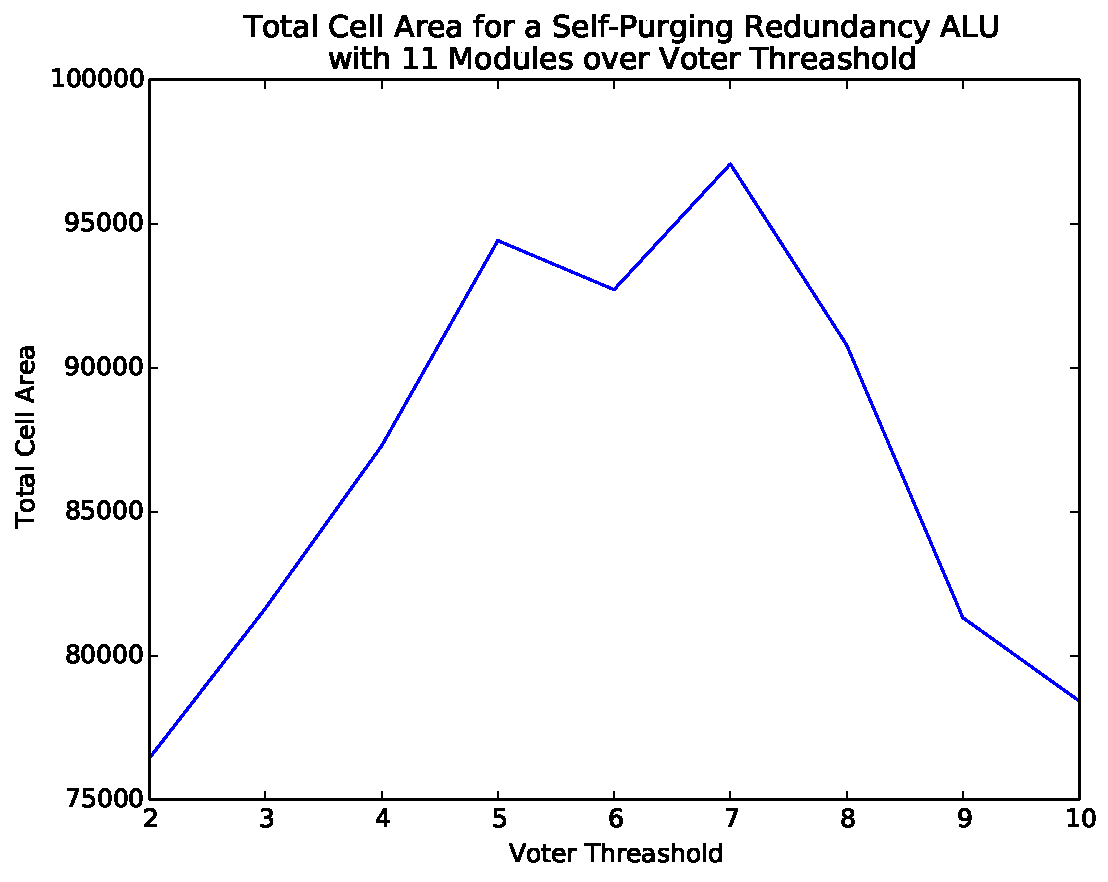
\includegraphics[width=0.5\textwidth]{area_11}

    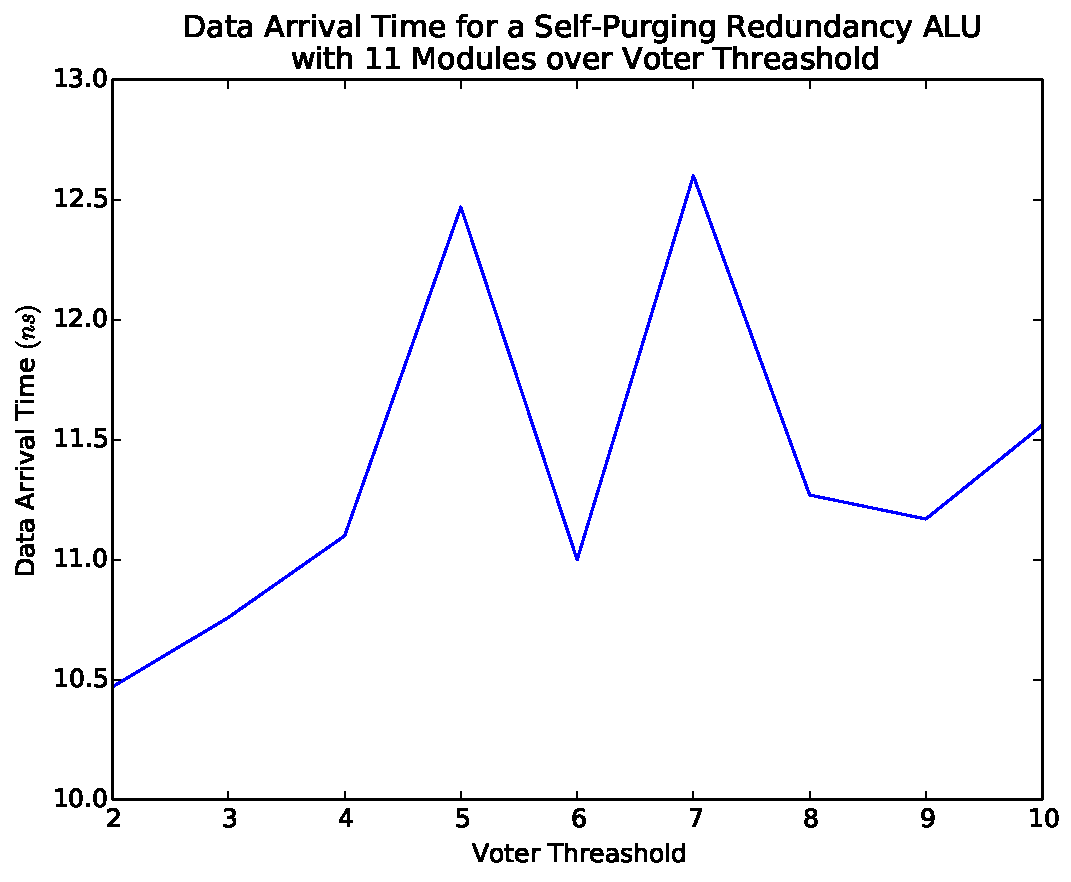
\includegraphics[width=0.5\textwidth]{time_11}
    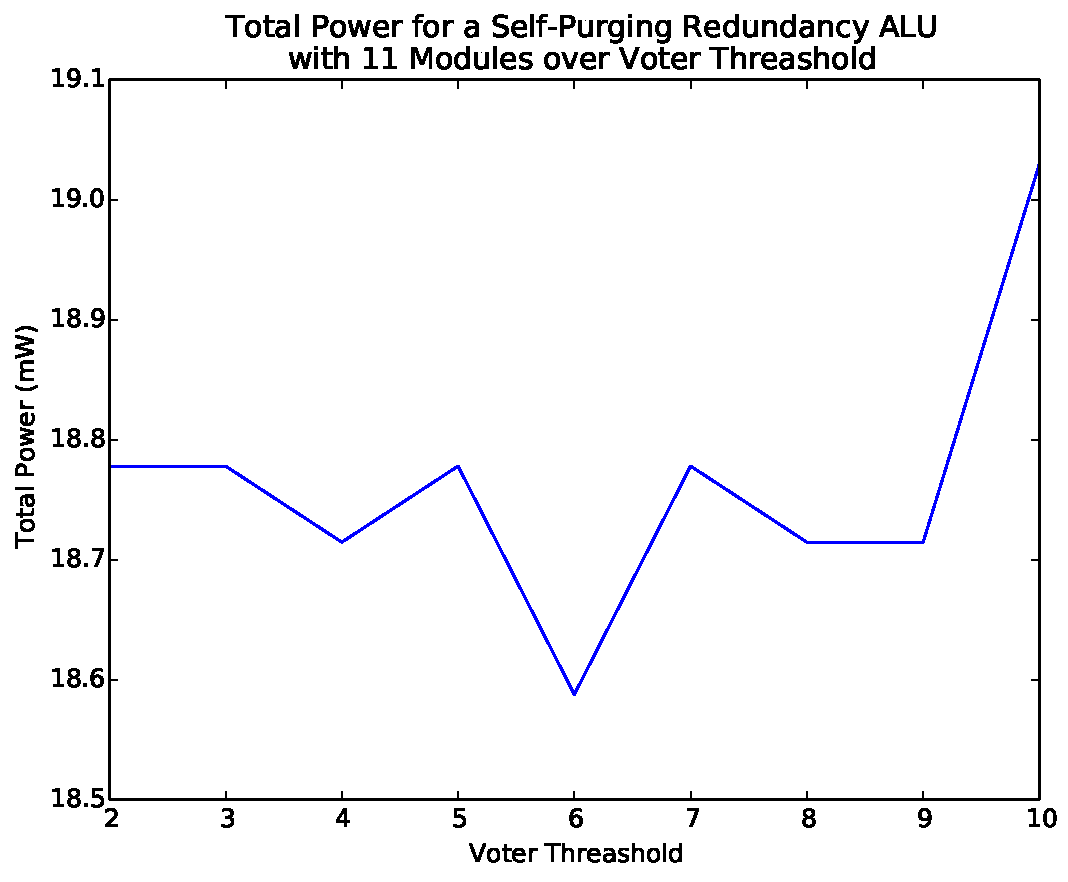
\includegraphics[width=0.5\textwidth]{power_11}

    Again, a voter threashold of 2 offers the best reliability, and has better area and timing than the others. The only case where it performs worse is power consumption. This would be an interesting point to investigate further, alongside why a threashold of six seems to have such good metrics.

    \subsection{Results for Different Number of Modules}

    Plotted below is the reliability for the ALU over time, using SPR with the number of modules ranging from 3 to 11 and a voter threashold of 2. Also displayed is the area, timing and power consumption. All of these are measured using the same techniques as in Section~\ref{subsec:threasholds}.

    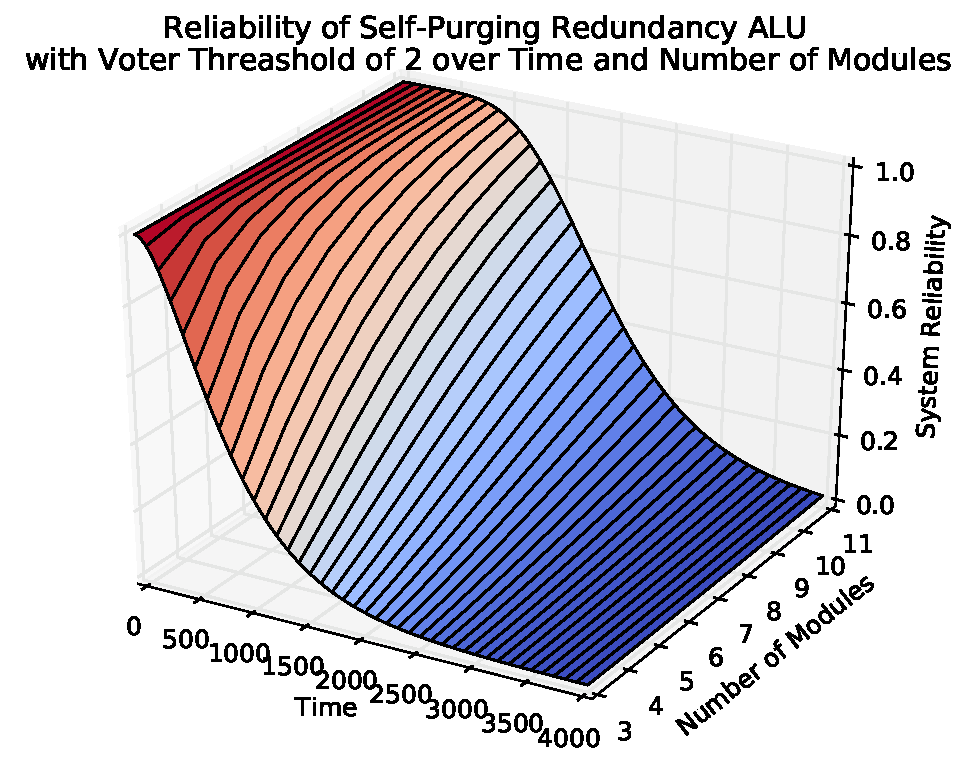
\includegraphics[width=0.5\textwidth]{reliability}
    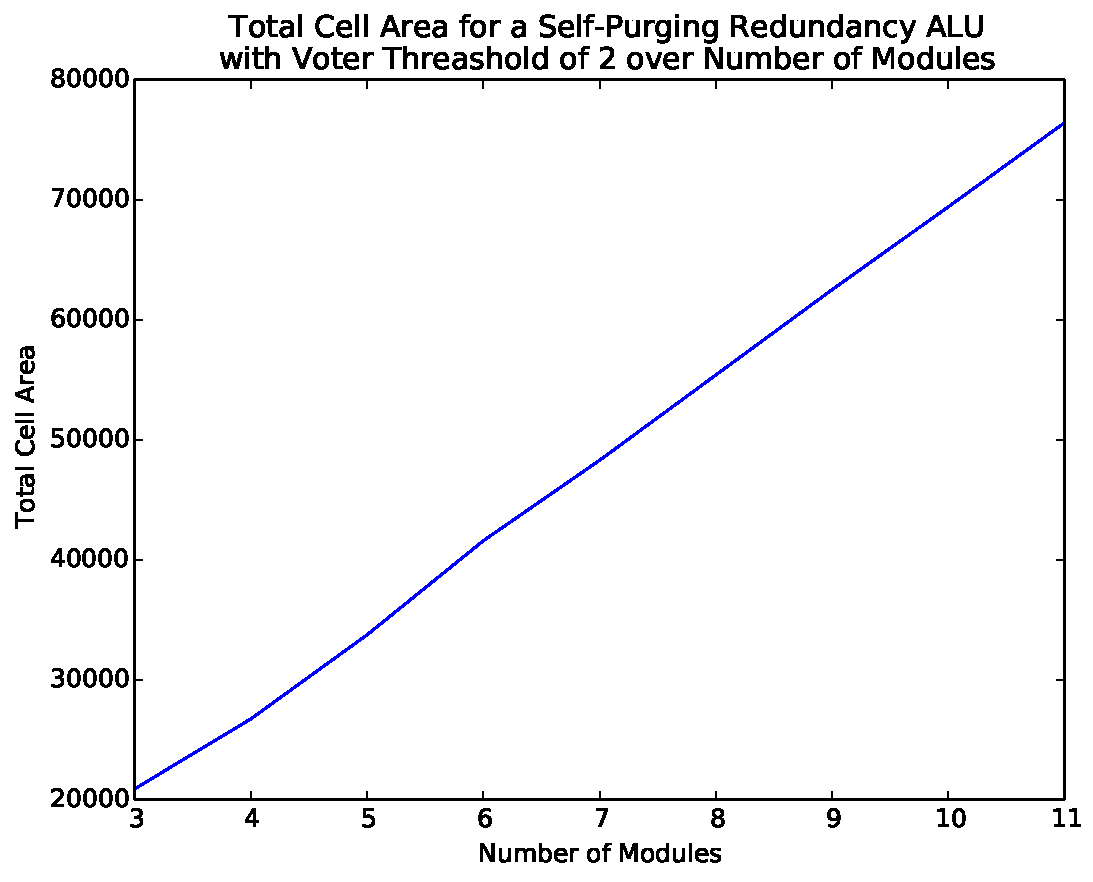
\includegraphics[width=0.5\textwidth]{area}

    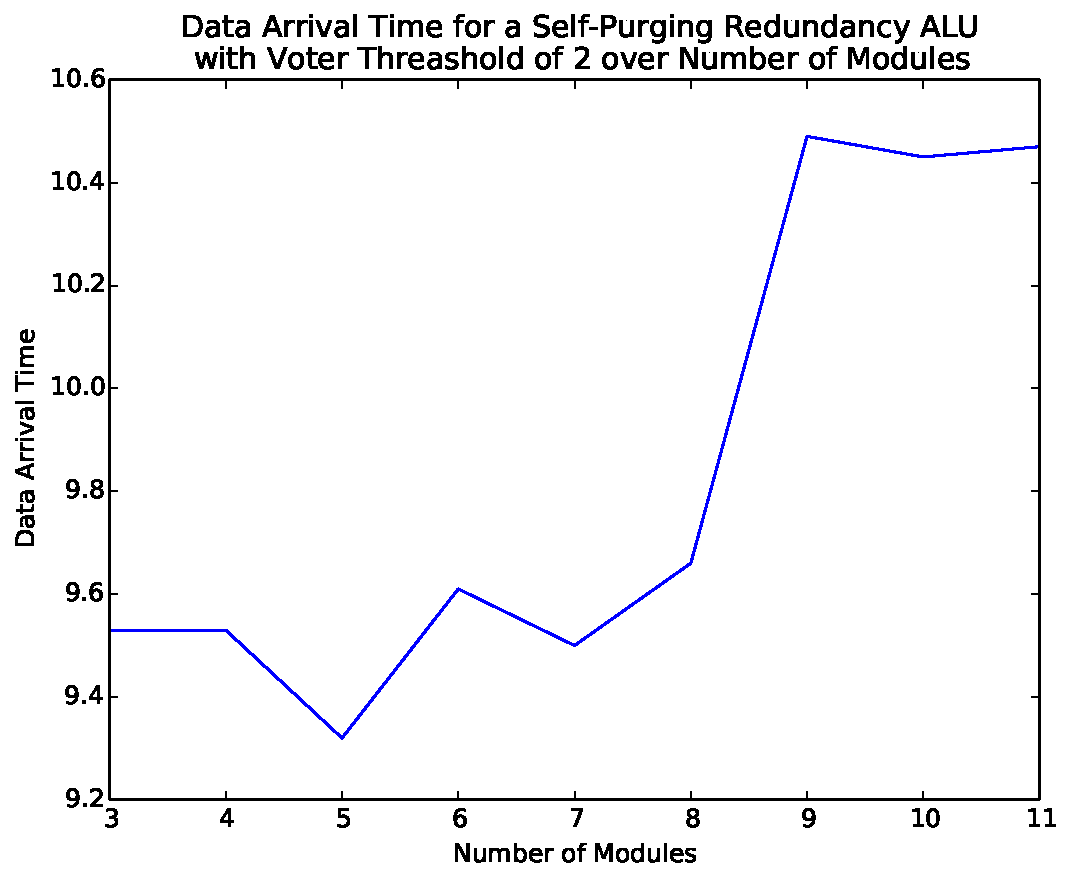
\includegraphics[width=0.5\textwidth]{time}
    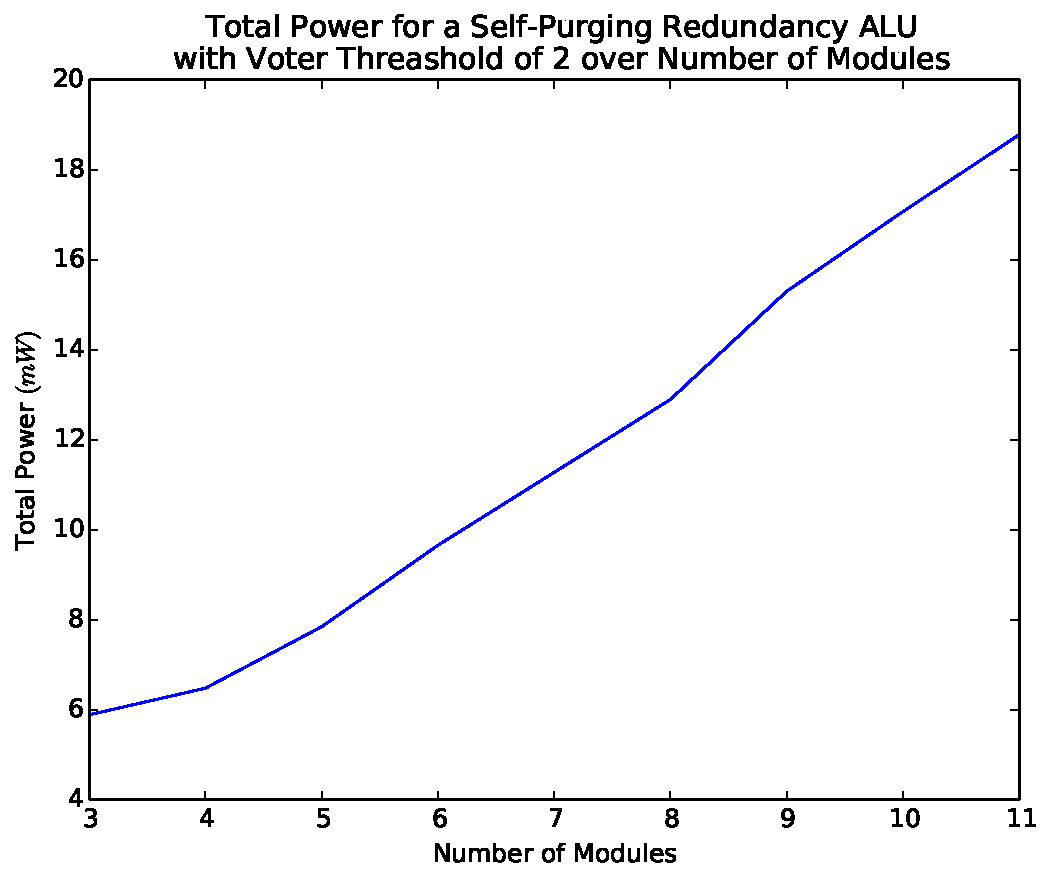
\includegraphics[width=0.5\textwidth]{power}

    This was more challenging to consider, as the reliability significantly increases with the number of modules, but so does the overheads.

    In the end, I selected five modules. Out of the circuits tested, it has the lowest data arrival time and one of the lower area and power demands. While it doesn't have the best reliability, the overhead was deemed not worthwhile.

    An interesting question is how the timing scales over the number of modules. While the other two metrics scale near-linearly -- which is expected as each module requires a constant amount of area and power -- time remains almost flat for the most part before suddenly jumping at 9 modules and then returning to almost flat. The likely explanation is that Design Compiler applies optimisations during synthesis, and this produces multiple levels of gates in the voter as the number of modules increases, as opposed to the two levels in the logic described in Section~\ref{sec:realisation}. We could test this by seeing if it jumps again if we increase the number of modules even further.

    \subsection{Performance in Comparison to the Original ALU}
    Tabled below is the performance of the 5 module SPR ALU in comparison to the original single ALU.

    \begin{tabular}{|c|c|c|c|}
        \hline
        & Original ALU & SPR ALU & Overhead \\ \hline
        Total Cell Area $(\mu m)$ & 4238.46 & 33752.87 & 7.96 \\ \hline
        Data Arrival Time $(f)$ & 8.60 & 9.32 & 1.08 \\ \hline
        Total Power $(mW)$ & 1.4923 & 7.8461 & 5.26 \\ \hline
    \end{tabular}

    N.B. Slack has not been recorded for this project, as neither circuit is driven by the system clock.

    The area and power consumption is significantly larger than that of the original ALU. This is expected, given that the SPR ALU consists of multiple copies of the original, plus the cost of the voter and switches.

    The timing overhead is larger than the original, but only relatively slightly. This is because the extra time for the voter is small for five modules.

    \subsection{Performance in Comparison to NMR}
    I also investigated how these circuits compared to NMR systems. The area, timing and power consumption are graphed below for 3, 5, 7, 9 and 11 modules.

    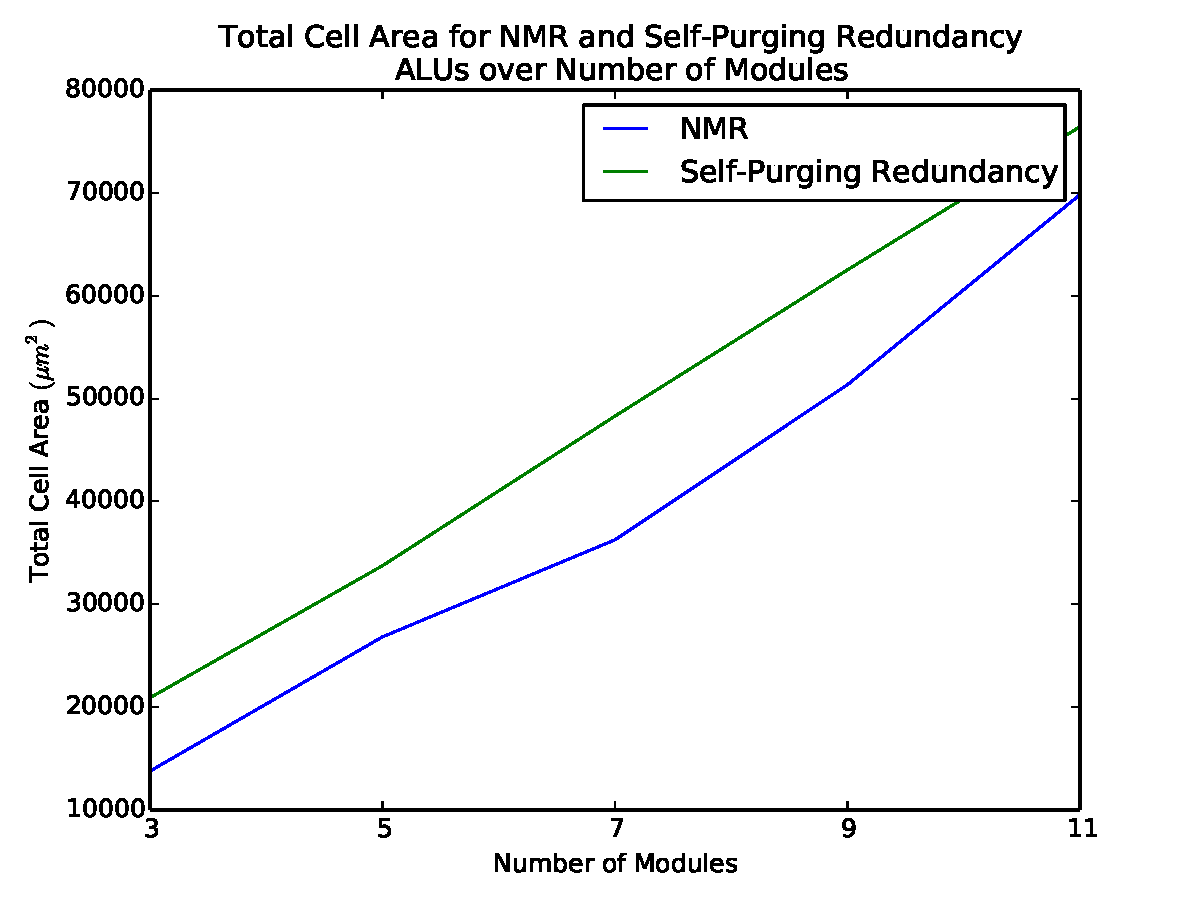
\includegraphics[width=0.5\textwidth]{area_nmr}
    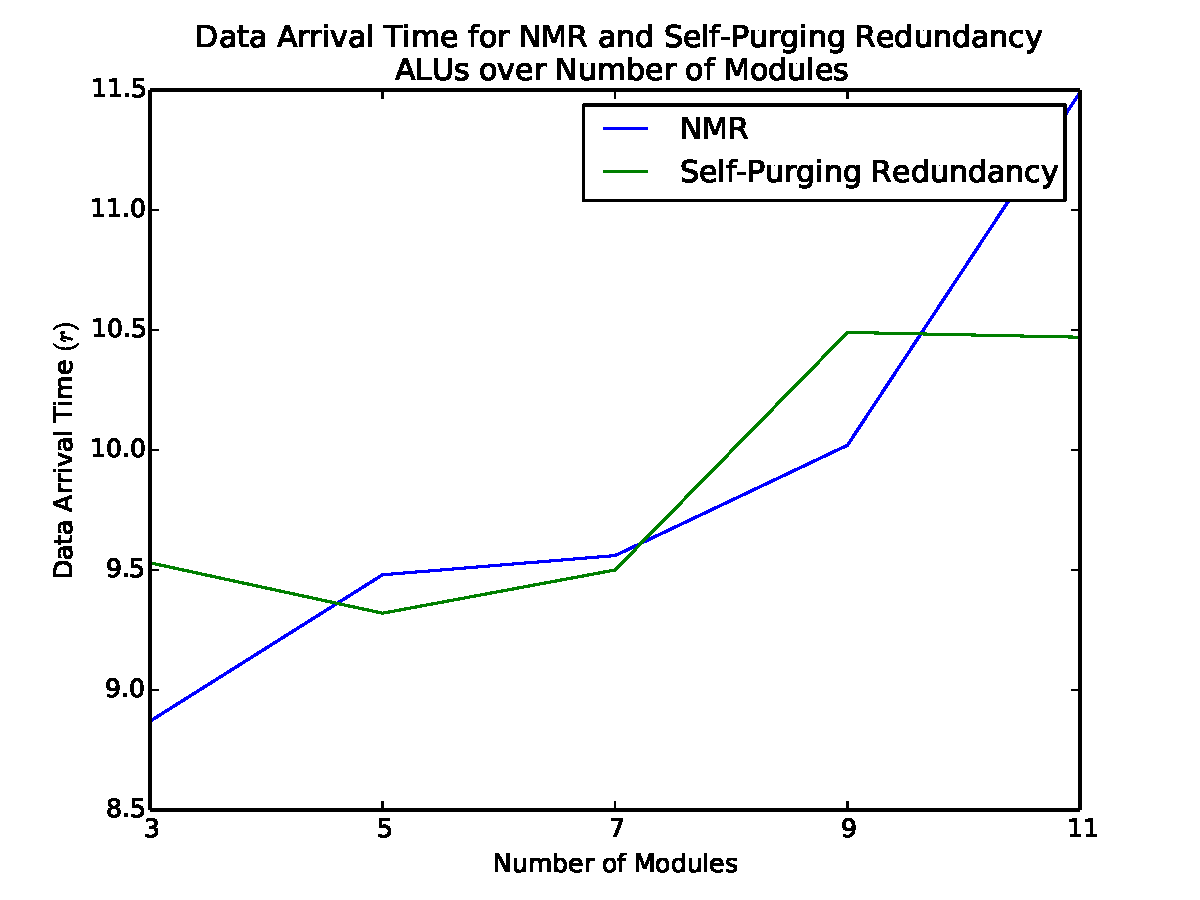
\includegraphics[width=0.5\textwidth]{time_nmr}

    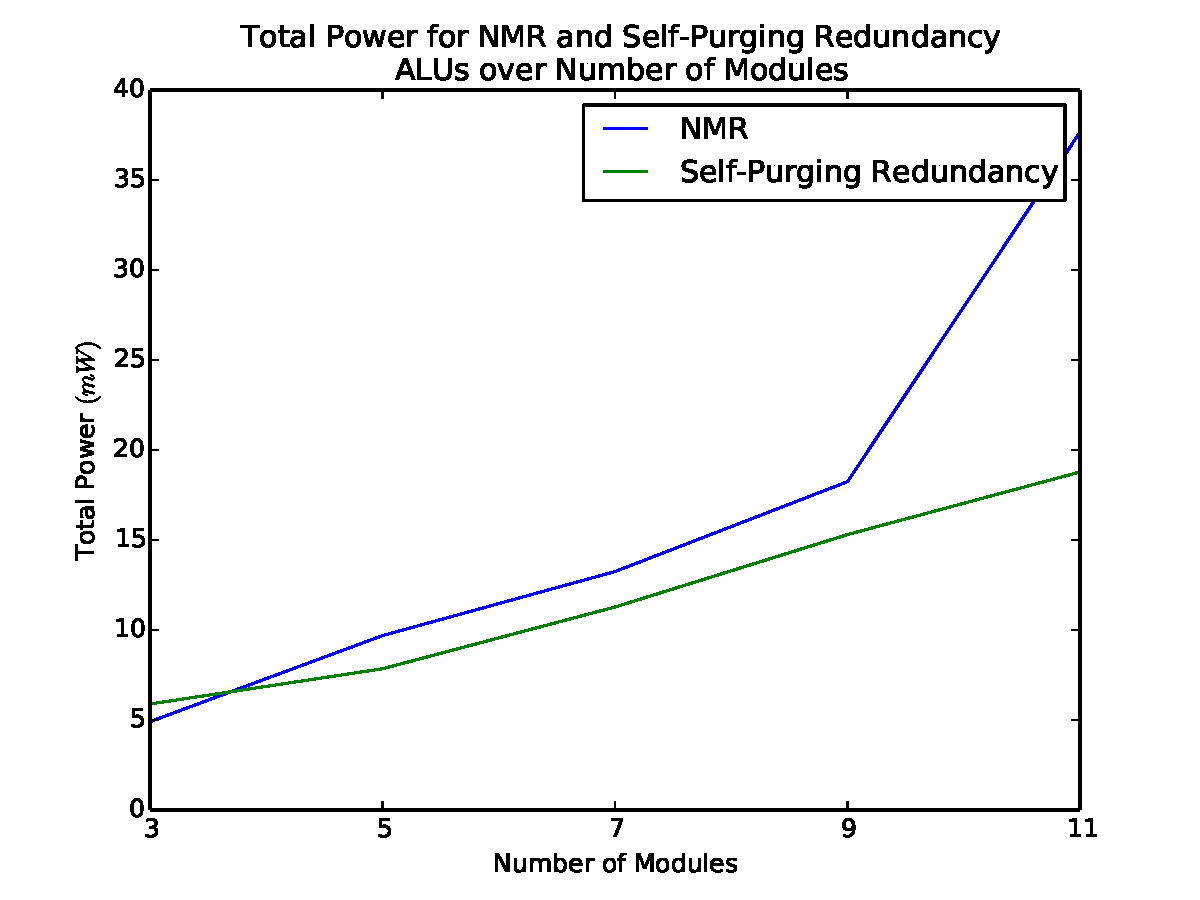
\includegraphics[width=0.5\textwidth]{power_nmr}

    An interesting observation is that with both timing and power consumption, NMR suddenly starts increasing dramatically at roughly 9 modules and continues at 11 modules. Even with area, we can see between 9 modules and 11 modules the gap between NMR and self-purging redundancy decreasing.

    The likely reason for this is that at nine modules, the complexity of the voter for NMR is starting to become the main overhead, instead of the modules. As the number of modules increases, NMR's voter becomes significantly more complex. This is because the threashold for NMR also needs to increase, to ensure that it is a majority verdict. SPR's voter on the other hand can always have a threashold of two. It will also become more complex as the number of modules increases, but more gradually than NMR's.

    \section{Lessons Learned}
    There are some interesting points to take away from this project.

    The first is that more redundancy is not necessarily better. While the reliability can increase with more instances, this comes with a dramatic overhead in terms of area, timing and power.

    The second is that SPR is more configurable than I initially thought, with the ability to set the threashold on the voter to any number of modules. While two modules is the standard setup, one interesting question is if there are cases where we would prefer a higher threashold. For example, if the voter threashold is two and two modules become faulty during the same operation then the whole system might fail.

    The third is that in some cases, NMR can be worse than SPR. This is particularly true in power consumption, and is largely due to the higher voter threashold in NMR. This might not necessarily hold true if we increase the threashold for self-purging redundancy, as discussed above.

    \section{Conclusion}
    In this project, I have made an ALU component of a MIPS processor fault tolerant by use of self-purging redundancy. This code is supplied in the submitted file mipsparts.v, and is commented with points to explain major components and points of interest.

    From synthesis, we can see that while SPR provides higher reliability, the area and power overhead is dramatic. For five extra modules, we require nearly eight times the area.

    Whether SPR is suitable for the ALU component in this MIPS processor depends on the application the processor will be used for. For commercial use, I would recommend against it; the area overhead in particular is far too large. For other failure-critical uses though, the increase in reliability could be worthwhile.

    \printbibliography

\end{document}
